\documentclass[tikz,border=8pt]{standalone}
\usepackage{pgfplots}
\usepgfplotslibrary{groupplots}
\pgfplotsset{compat=1.18}
\begin{document}
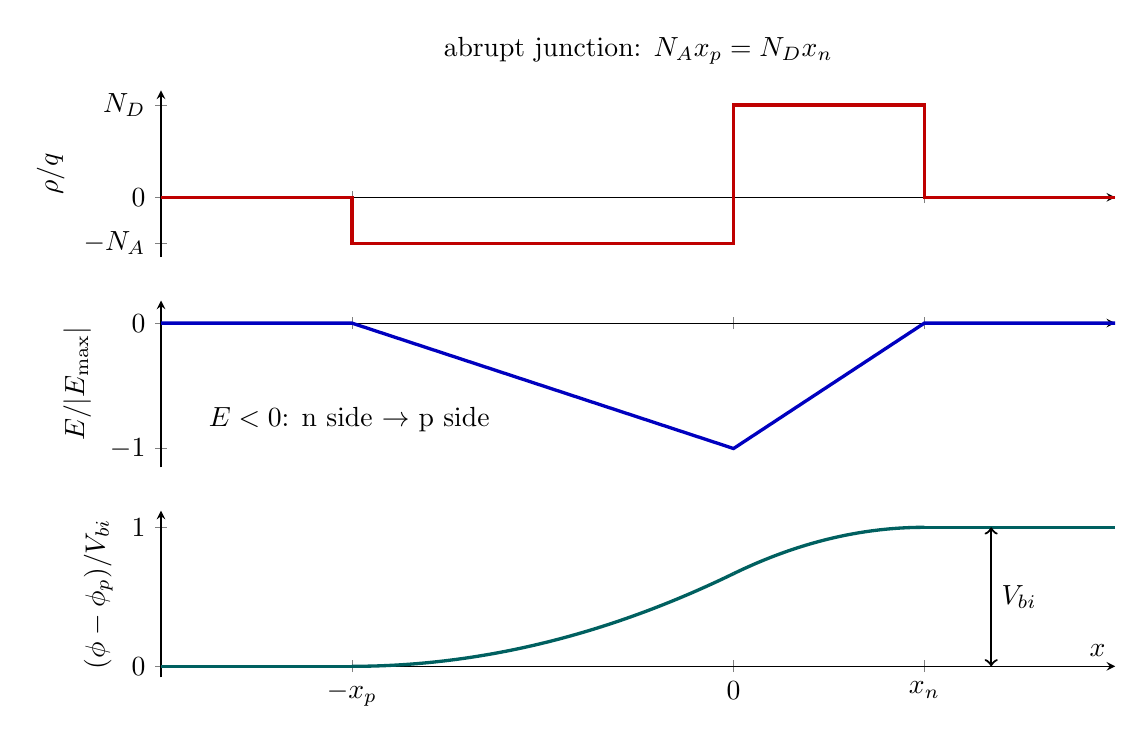
\begin{tikzpicture}
\begin{groupplot}[
  group style={group size=1 by 3,vertical sep=0.55cm},
  width=13.7cm,height=3.7cm,xmin=-3,xmax=2,
  axis x line=middle,axis y line=left,
  xtick={-2,0,1},xticklabels={$-x_p$,$0$,$x_n$},
  clip=false
]
\nextgroupplot[
  title={abrupt junction: $N_Ax_p=N_Dx_n$},
  ymin=-0.65,ymax=1.16,ylabel={$\rho/q$},
  ytick={-0.5,0,1},yticklabels={$-N_A$,$0$,$N_D$},xticklabels={}
]
\addplot[very thick,red!75!black] coordinates {(-3,0)(-2,0)(-2,-0.5)(0,-0.5)(0,1)(1,1)(1,0)(2,0)};
\nextgroupplot[
  ymin=-1.15,ymax=0.18,ylabel={$E/|E_{\max}|$},
  ytick={-1,0},xticklabels={}
]
\addplot[very thick,blue!75!black] coordinates {(-3,0)(-2,0)(0,-1)(1,0)(2,0)};
\node[anchor=west] at (axis cs:-2.8,-0.77) {$E<0$: n side $\to$ p side};
\nextgroupplot[
  ymin=-0.08,ymax=1.12,ylabel={$(\phi-\phi_p)/V_{bi}$},xlabel={$x$},
  ytick={0,1}
]
\addplot[very thick,teal!75!black,domain=-3:-2,samples=2]{0};
\addplot[very thick,teal!75!black,domain=-2:0,samples=100]{(x+2)^2/6};
\addplot[very thick,teal!75!black,domain=0:1,samples=100]{(1+x-x^2/2)/1.5};
\addplot[very thick,teal!75!black,domain=1:2,samples=2]{1};
\draw[<->,thick] (axis cs:1.35,0)--node[right]{$V_{bi}$}(axis cs:1.35,1);
\end{groupplot}
\end{tikzpicture}
\end{document}
